% ****** Start of file aipsamp.tex ******
%
%   This file is part of the AIP files in the AIP distribution for REVTeX 4.
%   Version 4.1 of REVTeX, October 2009
%
%   Copyright (c) 2009 American Institute of Physics.
%
%   See the AIP README file for restrictions and more information.
%
% TeX'ing this file requires that you have AMS-LaTeX 2.0 installed
% as well as the rest of the prerequisites for REVTeX 4.
%
% It also requires running BibTeX. The commands are as follows:
%
%  1)  latex  aipsamp
%  2)  bibtex aipsamp
%  3)  latex  aipsamp
%  4)  latex  aipsamp
%
% Use this file as a source of example code for your aip document.
% Use the file aiptemplate.tex as a template for your document.
\documentclass[%
 aip,
%jmp,%
%bmf,%
%sd,%
rsi,%
 amsmath,amssymb,
%preprint,%
 reprint,%
%author-year,%
%author-numerical,%
]{revtex4-1}

\usepackage{graphicx}% Include figure files
\usepackage{dcolumn}% Align table columns on decimal point
\usepackage{bm}% bold math
%\usepackage[mathlines]{lineno}% Enable numbering of text and display math
%\linenumbers\relax % Commence numbering lines

%\usepackage{caption}
\usepackage{subcaption}
\usepackage{cleveref}

\begin{document}

\preprint{AIP/123-QED}

\title[Sample title]{Evidence of terbium and oxygen co-segregation in annealed AlN:Tb}% Force line breaks with \\
%\thanks{Footnote to title of article.}

\author{V.C. Angadi}
\email{vcangadi1@sheffield.ac.uk}

\author{T. Walther}%
\email{t.walther@sheffield.ac.uk}

\affiliation{Dept. Electronic \& Electrical Eng., Kroto Centre for High-Resolution Imaging and Spectroscopy, University of Sheffield, North Campus, Wheeldon Street, Sheffield S3 7HQ, UK}

\author{F. Benz}
\affiliation{NanoPhotonics Centre, Cavendish Laboratory, Department of Physics, University of Cambridge, JJ Thomson Ave, Cambridge, CB3 0HE, United Kingdom}

\author{T. Aoki}
\affiliation{LeRoy Eyring Center for Solid State Science, Arizona State University, Tempe, AZ 85287, USA}

\date{\today}% It is always \today, today,
             %  but any date may be explicitly specified

\begin{abstract}
Analytical scanning transmission electron microscopy has been applied to study aluminium nitride (AlN) doped with terbium (Tb) and annealed at $800^\circ$C. Correlation of the maps of terbium and oxygen (O) from electron energy-loss spectrum image proves that these two elements co-segregate, replacing aluminium (Al) and nitrogen (N) atoms respectively. This agrees well with modelling which predicted the existence of Tb$-$O complexes to successfully fit the rather complicated cathodoluminescence emission spectra of the sample.

%Valid PACS numbers may be entered using the \verb+\pacs{#1}+ command.
\end{abstract}

\pacs{Valid PACS appear here}% PACS, the Physics and Astronomy
                             % Classification Scheme.
\keywords{aluminium nitride, terbium, segregation, luminescence, electron microscopy}
%Use showkeys class option if keyword
                              %display desired
\maketitle

\section{Introduction:}
\label{sec:Intro}
(general info on Tb emission spectra, luminescence, AlN, modelling, need for analytical STEM.)

\section{Experimental Details}
\label{sec:exp_detail}

\subsection{Growth + Anneal details}
\label{sec:growth}
(from Felix's thesis)

\subsection{Cathodoluminescence details}
\label{sec:CL}
(from thesis)

\subsection{STEM}
\label{sec:STEM}
All spectrum images (SI) have a field of view of $70nm$ and have been rotated through $\sim90^0$ so that the growth direction in all maps points upwards. AlN has been grown on top of Si substrate. AlN has been doped with 1-2\% of Tb and annealed.
\begin{table}
	\caption{EELS data acquisition parameters for the two spectrum 	images (SI) acquired from the same area.}
    \label{tab:Attributes}
	\begin{ruledtabular}
		\begin{tabular}{lll}
			Attributes&Low loss SI&High loss SI							\\ \hline
            Acceleration voltage (kV) &$60$&$60$						\\
			Spatial image size (pixels)&$87\times100$&$87\times100$ 	\\
            Real-space pixel size (\AA)&$7$&$7$							\\
            Spectrum channels		&$2048$&$512$						\\
			Dispersion (eV per channel)&$0.7$&$2.8$						\\
			Nominal field of view (nm) &$70$&$70$						\\
			Conv. angle ($\alpha$)(mrad)&$30$&$30$						\\
			Coll. angle ($\beta$)(mrad)&$45$&$45$						\\
			Spectrum offset (eV)&$0$&$310$								\\
			Exposure time (seconds)&$8\times10^{-5}$&$1\times10^{-1}$	\\
			Total acquisition time &$\sim700ms$&$\sim14m~30s$
		\end{tabular}
	\end{ruledtabular}
\end{table}
%\section{Low loss Spectrum image (SI) analysis}
%\label{sec:SI_analysis}
An annular dark-field (ADF) image is shown in Fig.~\ref{fig:HAADF}. The vertical lines in the ADF image are artefacts due to emission current fluctuations of the cold field emitter electron gun. A relative thickness map is shown in fig.~\ref{fig:tl}. The acquisition parameters of two EELS SI are listed in Table~\ref{tab:Attributes}. The inelastic mean free path ($\lambda$) values in Si (substrate), AlN:Tb region and SiO$_2$ region are $\approx49nm$, $\approx52nm$ and $\approx54nm$ respectively (reference to Egerton calculation). The values of the relative thickness ($t/\lambda$) map can thus be directly related to absolute specimen thickness ($t$) in the range of $13-20nm$.
\begin{table}
	\caption{Calculated mean free path ($\lambda$)}.
    \label{tab:lambda}
    \begin{ruledtabular}
    	\begin{tabular}{lccc}
        	Composition&Al:N:Tb:O&Si:O&Si:O										\\
            at.\%&$48:49:2:1$&$33.3:66.7$&$99:1$								\\ \hline
        	$\langle \text{Z} \rangle$&$11.05$&$10.00$&$13.94$					\\
            $\langle \text{A} \rangle$&$23.15$&$20.03$&$27.97$					\\
            $\langle \text{E} \rangle~\left[eV\right]$&$18.0$&$17.4$&$19.6$		\\
           	$\lambda~\left[nm\right]$&$52.4$&$54.0$&$48.9$
    	\end{tabular}
    \end{ruledtabular}
\end{table}
For calculation of $t/\lambda$, the intensity of the spectra up to the minimum between zero-loss peak and plasmon peak is approximated as the intensity of the zero-loss ($I_0$). Hence $I_0$ contains not only zero-loss intensity, but also phonon losses, retardation and \v{C}erenkov losses etc. The total intensity ($I_t$) also contains, inter-band transitions, plasmon losses and ionization core-losses. Hence the $t/\lambda$ values calculated as per eqn.~\ref{eq:tl} will always be slight over-estimates (fig.~\ref{fig:tl}). More accurate ways to measure $t/\lambda$ would include fitting the bulk plasmon with a Lorentz function $L(E,E_p,W_p)$ (eqn.~\ref{eq:lorentz}) and the monochromated zero-loss with a Gaussian function $G(E,E_0,W_0)$ (eqn.~\ref{eq:gauss}) and weighting both according to a Poisson distribution $P(n,t/\lambda)$ simultaneously as shown in eqns.~\ref{eq:poisson} \& \ref{eq:low_loss}.
\begin{eqnarray}
	t/\lambda = \operatorname{ln}\left(\frac{I_t}{I_0}\right)
    \label{eq:tl}
\end{eqnarray}
\begin{eqnarray}
	P(n,t/\lambda) = \left(\frac{t}{\lambda}\right)^n\left(\frac{1}{n!}\right)\operatorname{exp}\left(-\frac{t}{\lambda}\right)
    \label{eq:poisson}
\end{eqnarray}
\begin{eqnarray}
	L(E,E_p,W_p) = \frac{A_p}{\pi} \frac{\frac{1}{2}W_p}{(E-E_p)^2+\left(\frac{1}{2}W_p\right)^2}
    \label{eq:lorentz}
\end{eqnarray}
\begin{eqnarray}
	G(E,E_0,W_0) &=& \frac{A_0}{\sqrt{\pi}}\frac{2\sqrt{\operatorname{ln}~2}}{W_0}\nonumber\\
    & & \times \operatorname{exp}\left(-\left[(E-E_0)\frac{2\sqrt{\operatorname{ln}~2}}{W_0}\right]^2\right)
    \label{eq:gauss}
\end{eqnarray}
\begin{eqnarray}
	S(E,t/\lambda,E_0,W_0,E_p,W_p) = P(0,t/\lambda)~G(E,E_0,W_0) \nonumber \\
     +\sum_{k=1}^{n}P(k,t/\lambda)~L(E,k\times E_p,W_p) \nonumber \\
    \label{eq:low_loss}
\end{eqnarray}
where $n = \lfloor E_{max}/E_p \rfloor \in \mathbb{N}$.  $t/\lambda$, position ($E_0$) and full width at half maximum (FWHM) ($W_0$) of the zero-loss peak, position ($E_p$) and FWHM ($W_p$) of bulk plasmon are the fitting parameters. Eqn.~\ref{eq:tl} can be used as an initial estimate of $t/\lambda$ in multiple linear least squares (MLLS) fit of low loss in eqn.~\ref{eq:low_loss}. This can be extended to the entire SI which provides more accurate $t/\lambda$ values. Figs.~\ref{fig:Ep_map} and \ref{fig:Wp_map} are maps of $E_p$ and $W_p$ obtained from eqn.~\ref{eq:lorentz} where the values of the plasmon peak energy have been interpolated to sub-pixel precision ($\approx$0.1eV).

\section{CL spectroscopy}
\label{sec:CLS}

\section{Modelling}
\label{sec:model}
To further investigate the surroundings of Tb$^{3+}$ ions, we have performed simulations of an AlN supercell (consisting of 18 AlN unit cells) using MOPAC2012 \cite{steward12} with the extension SPARKLE \cite{freire10} to describe the rare-earth ion. For pure, undoped, AlN we found good agreement between the lattice constants of AlN predicted by our simulation (a = 3.12\AA; c = 5.05\AA) and previous reports (a = 3.11\AA; c = 4.98\AA) \cite{ICDD11}. Subsequently, we have replaced an Al$^{3+}$ ion with a Tb$^{3+}$ one, three N$^{3-}$ by O$^{2-}$, and another Al$^{3+}$ by a vacancy to ensure charge neutrality. Initially we distributed these lattice defects within the supercell so that they are spaced far apart and calculated the energy of formation of this 'random' state as our reference energy. We systematically varied the local arrangement, optimised the geometry, and compared the resulting energies of formation. We find that placing the oxygen ions in the nearest neighbouring positions of the terbium ion leads to an energy increase of around 2.5eV per supercell. In contrast, if the aluminium vacancy V$_\text{Al}$ is placed next to the terbium ion we find that the energy of formation is reduced by -1.38eV. This reduction is likely due to the release of strain energy which is introduced by the larger atomic radius of the Tb$^{3+}$ ion compared to the Al$^{3+}$ one. Gradually coordinating the aluminium vacancy with more and more oxygen ions leads to a further degrease in energy (-4.98eV). The geometry of this lowest energy state is shown in fig.~\ref{fig:felix_model}a. We denote these complexes according to the coordination of the vacancy, for instance the lowest energy one as (V$_\text{Al}$)(O)$_3$(NTb). Fig.~\ref{fig:felix_model}b shows an overview of the energies of different V$_\text{Al}-$N$-$Tb complexes (see SI for illustrations of the geometry of all complexes). Probably these complexes are formed during the annealing procedure, which is necessary to 'activate' the rare-earth luminescence.
\begin{figure}
	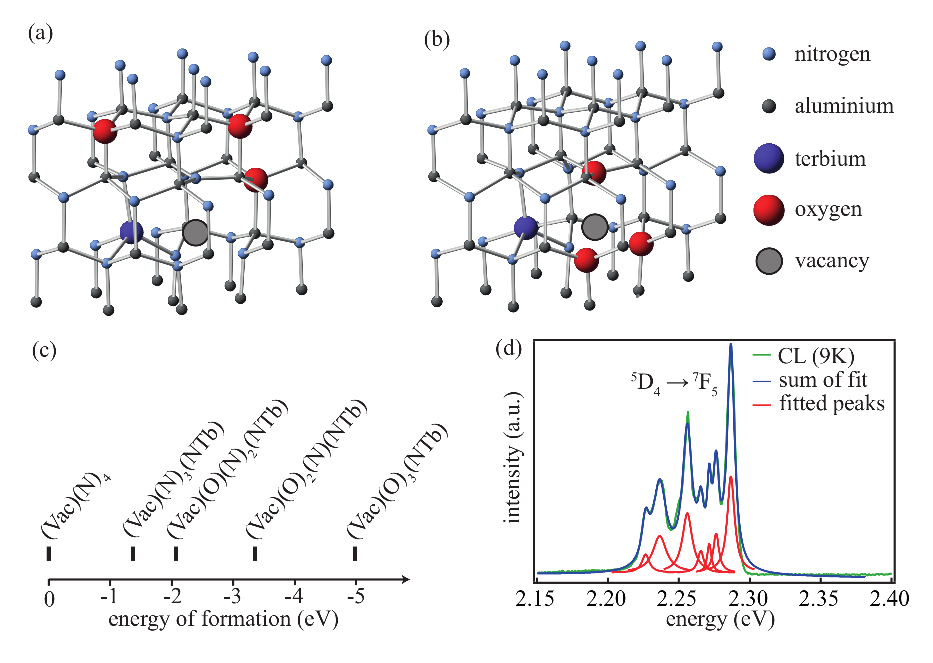
\includegraphics[width=0.4\textwidth]{model}
    \caption{(a)~Illustration of the lowest energy Tb$^{3+}$ complex. (b)~Comparison of the energies of formation of different Tb-N-V$_\text{Al}$ complexes. The names show the four nearest neighbours of the aluminium vacancy. (c)~High resolution cathodoluminescence spectrum of the $^5$D$_4$ to $^7$F$_5$ transition of Tb$^{3+}$ ions incorporated in AlN.}
    \label{fig:felix_model}
\end{figure}
From the fully relaxed structure we find a reduction of the local symmetry of the Tb$^{3+}$ lattice site from T$_\text{d}$ to C$_\text{3v}$, corresponding to a slight change in the bond length along one direction of the coordination tetrahedron. To verify this reduction in symmetry we have recorded cathodoluminescence spectra of the $^5$D$_4$ to $^7$F$_5$ transition of the trivalent terbium ions at 4K (see fig.~\ref{fig:felix_model}c). This transition reveals a seven-fold splitting of the $^7$F$_5$ energy level, which is consistent with the expected number of states in the case of the C$_\text{3v}$ symmetry (for T$_\text{d}$ only four states would be expected) \cite{henderson05}.

\section{STEM EELS SI}
\label{sec:STEMEELSSI}
The elemental maps are shown in Fig.~\ref{fig:elemental_maps}. The background fitting details are listed in Table~\ref{tab:back_fit_table} along with the integration range ($\Delta$). The functions used to fit the background are exponential decay (eqn.~\ref{eq:exp_fun}) or inverse power-law functions (eqn.~\ref{eq:pow_law}).
\begin{eqnarray}
	f(E) =
    \sum^{j=k}_{j=1}
    \left[
    \begin{array}{c}
    	A_1 	\\
        . 		\\
        . 		\\
        A_j 	\\
    \end{array}
    \right]
    \operatorname{exp}\left(-\left[
    \begin{array}{c}
    	r_1 	\\
        . 		\\
        . 		\\
        r_j 	\\
    \end{array}
    \right]E\right)
    \label{eq:exp_fun}
\end{eqnarray}
\begin{eqnarray}
	f(E) = AE^{-r}
    \label{eq:pow_law}
\end{eqnarray}
\begin{table}
	\caption{Background fitting details. All numerical values are in eV.}
    \label{tab:back_fit_table}
    \begin{ruledtabular}
    	\begin{tabular}{lllllll}
    		SI	&edge	 &fit begin&fit end&onset&$\Delta$&fit type 	\\ \hline
            low loss&$Al~L_{2,3}$& $23.8$&$70$&$72.8$&$27.3$&$Exp2$\footnote{Superposition of two exponential decay functions (eqn.~\ref{eq:exp_fun}).} 		\\
            		&$Si~L_{2,3}$&$41.3$&$98$&$99.4$&$105$&$Exp2$ 			\\ \hline
            high loss&$N~K$&$343.6$&$385.6$&$385.6$&$112$&$Pow$\footnote{Inverse power-law function (eqn.~\ref{eq:pow_law})} 			\\
                	&$O~K$&$427.6$&$517.2$&$525.6$&$112$&$Exp1$\footnote{Exponential decay function (eqn.~\ref{eq:exp_fun}).} 			\\
            		&$Tb~M_{4,5}$&$727.2$&$1147.2$&$1211.6$&$246.4$&$Exp1$ 	\\
    	\end{tabular}
    \end{ruledtabular}
\end{table}
The value of $k = 1$ for fit type "$Exp1$", but $k = 2$ for fit type "$Exp2$" and Eqn~\ref{eq:pow_law} for fit type "$Pow$" as indicated in Table~\ref{tab:back_fit_table}. The Si L$_{2,3}$ edge and Al L$_{2,3}$ core-losses are extracted from low loss SI. N K, O K, Tb M$_{4,5}$ edges are extracted from high loss SI. The integration range ($\Delta$) for Al L$_{2,3}$ is limited by overlay with the Si L$_{2,3}$ edge. The maps of Al L$_{2,3}$ and Si L$_{2,3}$ (fig.~\ref{fig:qAlMap} \& \ref{fig:qSiMap}) are relatively noisy due to low exposure time and hence low signal to noise ratio (SNR). Large negative values in Si L$_{2,3}$ map are due to poor background fitting in the AlN region due to the preceding Al L$_{2,3}$ ionization edge. Deconvolution is not applied because of low SNR in the spectrum. Deconvolution with both Fourier-ratio or Richardson-Lucy (RL) methods would increase the noise even further. The interface in the high loss maps (\cref{fig:qNMap,fig:qOMap,fig:qTbMap}) appears to be inclined w.r.t the horizontal by an angle of $\approx4.65^\circ$ due to drift during the long exposure time while acquisition. Due to this mismatch in the interface, the atomic \% has been calculated only in the regions indicated in fig.~\ref{fig:40x87}. The FWHM  ($W_p$) of bulk plasmons (fig.~\ref{fig:Wp_map}) of oxides are known to be wider (refer). The evidence of drifting can be seen in O K map (map from high loss) (fig.~\ref{fig:qOMap}) and $W_p$ map (fig.~\ref{fig:Wp_map}).
\begin{figure}
	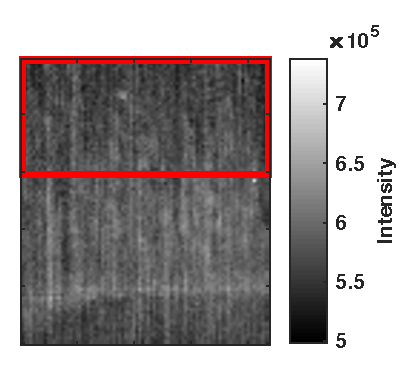
\includegraphics[scale=0.75]{40x87_region}
    \caption{Marked box in the AlN region for the calculation of elemental map correlations.}
    \label{fig:40x87}
\end{figure}
\begin{table}
	\caption{Elemental quantification (at\%) in AlN:Tb region for top 40 rows}
    \label{tab:atper}
    \begin{ruledtabular}
    	\begin{tabular}{ccccccc}
        	Region&Al&N&Tb&O&Si	\\ \hline
            AlN:Tb\&O&$43.17$&$38.66$&$1.40$&$15.78$&$0.01$ \\
            Si\&O &$17.20$&$0$&$0.80$&$20.30$&$62.34$
    	\end{tabular}
    \end{ruledtabular}
\end{table}

\section{Discussion} %(Anti) correlation of elemental maps
\label{sec:discussion}
In case of N K and O K (\cref{fig:qNMap,fig:qOMap}), the contrast of the maps indicate anti-correlation i.e. in the AlN region, oxygen is replacing nitrogen (group V). Terbium must be replacing aluminium in the group III sub-lattice. Although the corresponding decrease in local Al contrast is too small to become visible in fig.~\ref{fig:qAlMap}. Table.~\ref{tab:xcorr} lists the cross-correlation values between the elemental maps in the top half of AlN marked in fig.~\ref{fig:40x87}. The cross correlation of nitrogen and terbium map is negative (between $0$ to $-1$). Similar observations can be made between nitrogen and oxygen. The cross-correlation between terbium and oxygen with positive cross correlation.  indicating formation of Tb-O complexes.
\begin{table}
	\caption{Cross correlation between elemental maps in $AlN$ region marked by box in fig.~\ref{fig:40x87}.}
    \label{tab:xcorr}
    \begin{ruledtabular}
    	\begin{tabular}{cccccccc}
        	$X_{corr}$&Al&N&Tb&O&Si													\\ \hline
            Al& $1.0000$& $0.0802$& $0.0337$& $0.0012$&$-0.0920$					\\
             N& $0.0802$& $1.0000$& $\textbf{-0.0366}$&$\textbf{-0.3694}$&$-0.0060$	\\
            Tb& $0.0337$&$-0.0366$& $1.0000$& $\textbf{0.3466}$&$0.0064$			\\
             O& $0.0012$&$-0.3694$&	$0.3466$& $1.0000$&$0.0188$						\\
            Si&$-0.0920$&$-0.0060$&$0.0064$&$0.0188$& $1.0000$
    	\end{tabular}
    \end{ruledtabular}
\end{table}

\begin{figure*}
	\centering
    \begin{subfigure}{0.3\textwidth}
    	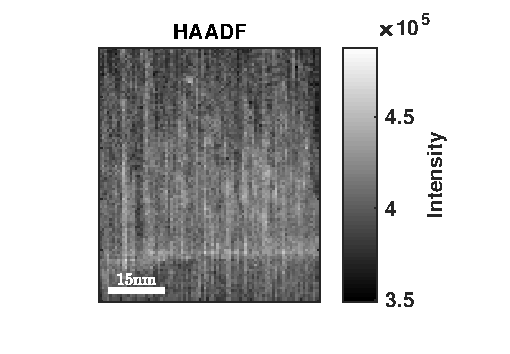
\includegraphics[width=\textwidth]{HAADF_SI1}
        \subcaption{}
		\label{fig:HAADF}
    \end{subfigure}
    \begin{subfigure}{0.3\textwidth}
		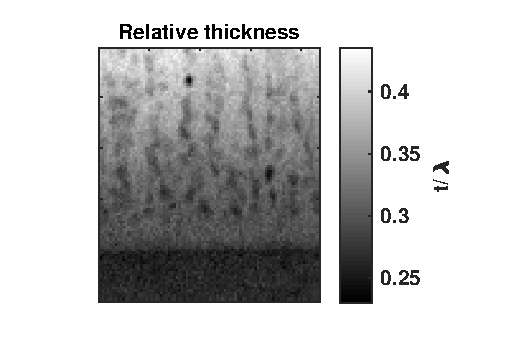
\includegraphics[width=\textwidth]{relative_thickness_map_SI1}
		\subcaption{}
		\label{fig:tl}
	\end{subfigure}
    
    \begin{subfigure}{0.3\textwidth}
		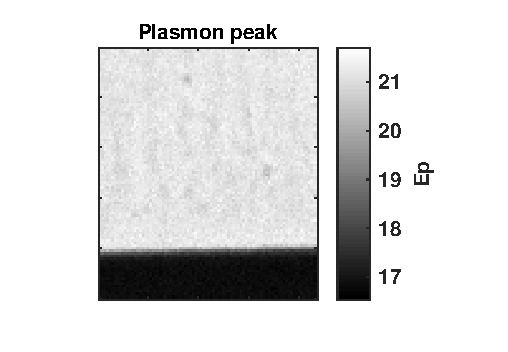
\includegraphics[width=\textwidth]{Ep_map_SI1}
		\subcaption{}
		\label{fig:Ep_map}
	\end{subfigure}
    \begin{subfigure}{0.3\textwidth}
		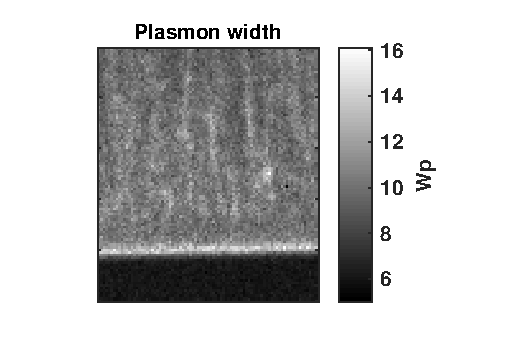
\includegraphics[width=\textwidth]{Wp_map_SI1}
		\subcaption{}
		\label{fig:Wp_map}
	\end{subfigure}
    \caption{(a)~HAADF and maps of (b)~relative thickness, (c)~plasmon peak energy, (d)~plasmon width.}
\end{figure*}

%\subsubsection{\label{sec:level3}Third-level heading: Citations and Footnotes}

\begin{figure*}
	\centering
    \begin{subfigure}{0.3\textwidth}
    	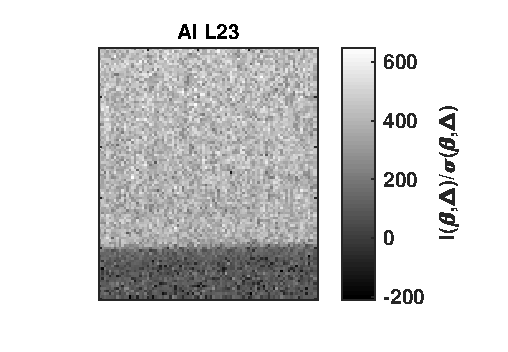
\includegraphics[width=\textwidth]{qAlMap}
        \subcaption{}
        \label{fig:qAlMap}
    \end{subfigure}
    \begin{subfigure}{0.3\textwidth}
    	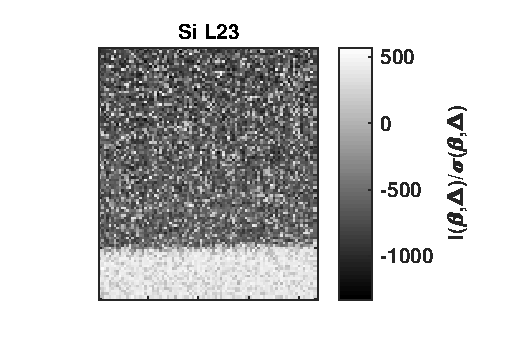
\includegraphics[width=\textwidth]{qSiMap}
        \subcaption{}
        \label{fig:qSiMap}
    \end{subfigure}
    
	\begin{subfigure}{0.3\textwidth}
    	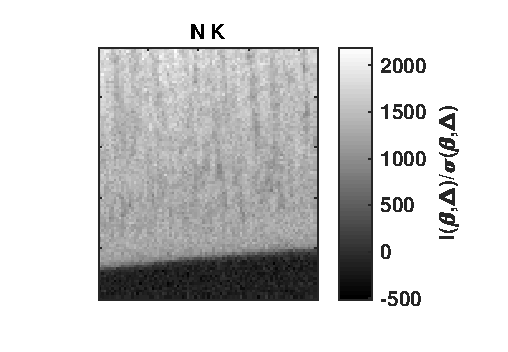
\includegraphics[width=\textwidth]{qNMap}
        \subcaption{}
        \label{fig:qNMap}
    \end{subfigure}
    \begin{subfigure}{0.3\textwidth}
    	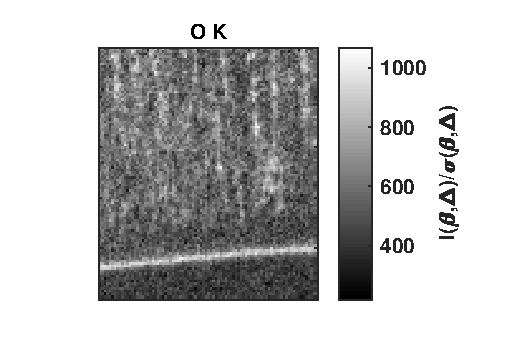
\includegraphics[width=\textwidth]{qOMap}
        \subcaption{}
        \label{fig:qOMap}
    \end{subfigure}
    \begin{subfigure}{0.3\textwidth}
    	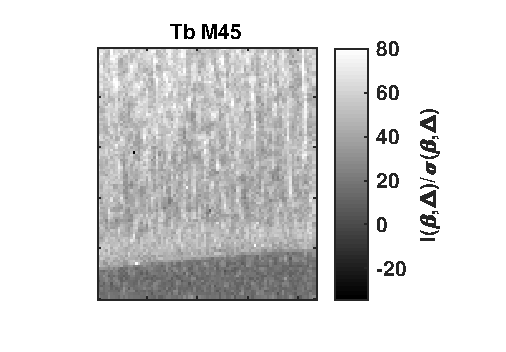
\includegraphics[width=\textwidth]{qTbMap}
        \subcaption{}
        \label{fig:qTbMap}
    \end{subfigure}
    \caption{Background subtracted intensities after the edge onset have been integrated and normalised w.r.t the corresponding scattering cross-sections and exposure times. (a,b)~Elemental maps of Al L$_{2,3}$ and Si L$_{2,3}$ in the low loss region. (c,d,e)~Elemental maps of N K, O K and Tb M$_{4,5}$ in the high loss region.}
    \label{fig:elemental_maps}
\end{figure*}

%\paragraph{Fourth-level heading is run in.}%

\begin{acknowledgments}
xyz
\dots.
\end{acknowledgments}

%\nocite{*}
\bibliography{aipsamp}% Produces the bibliography via BibTeX.

\end{document}
%
% ****** End of file aipsamp.tex ******